\documentclass{jarticle}
\usepackage{multicol}
\usepackage{bm}
\usepackage{amsmath}
\usepackage{amssymb}
\usepackage{color}
\usepackage{comment}
\usepackage[dvipdfmx]{graphicx}
\usepackage{listings}
%ここからソースコードの表示に関する設定
\lstset{
  basicstyle={\ttfamily},
  identifierstyle={\small},
  commentstyle={\smallitshape},
  keywordstyle={\small\bfseries},
  ndkeywordstyle={\small},
  stringstyle={\small\ttfamily},
  frame={tb},
  breaklines=true,
  columns=[l]{fullflexible},
  numbers=left,
  xrightmargin=0zw,
  xleftmargin=3zw,
  numberstyle={\scriptsize},
  stepnumber=1,
  numbersep=1zw,
  lineskip=-0.5ex
}

\makeatletter
\newenvironment{tablehere}
  {\def\@captype{table}}
  {}

\newenvironment{figurehere}
  {\def\@captype{figure}}
  {}
\makeatother

\begin{document}
\setcounter{section}{0}
\section{ガウス過程とは}
ガウス過程とは,関数を生成する確率分布である。
畳み込みニューラルネットワーク(convolutional neural network:CNN)について説明する。これは画像認識や音声認識など,いたるところで利用されている。
\subsection{全体の構造}
これまで見てきたNNは隣接する層のすべてのニューロン間で結合があった(全結合)。これをAffineレイヤという名前で実装した。この構造を図示すると以下のようになる。つまりAffineレイヤと活性化関数のレイヤを交互に通過するという構造である。\\
\scalebox{0.6}{\input{fig07-01.wtp}}

一方CNNの構造は以下のようになる。新しくConvolutionレイヤとPoolingレイヤが加わる。また特に注目する点としては,出力に近い層ではこれまでのAffine-ReLUやAffine-Softmaxという組み合わせが用いられる。
\scalebox{0.6}{\input{fig07-02.wtp}}

\subsection{畳み込み層}
CNNにおいては各層を流れるデータは形状のあるデータになるという点で,全結合のネットワークとは異なる。
\subsubsection{全結合層の問題点}
全結合層の問題点はデータの形状が無視されてしまうことにある。たとえば入力データが画像の場合,縦方向,横方向,チャンネル方向の$3$次元の形状を持っている。しかし全結合層への入力としては$1$次元のデータに変形する必要があった。これは例えば画像データであれば,近くのピクセルの値は近いなどといった重要な情報を無視することになっており,これを活かすことができない。\\
CNNにおいては畳み込み層の入出力データを特徴マップという。さらに,畳み込み層の入力データを入力特徴マップ,出力データを出力特徴マップという。
\subsubsection{畳み込み演算}
畳み込みは入力データに対してフィルター(カーネル)を適用することによって行われる。入力をサイズ$(H,W)$の行列$A$とし,フィルターをサイズ$(FH,FW)$の行列$B$とする。このとき
\[
X \circledast F = Y
\]
によって表現される畳み込み演算は
\[
y_{ij} = \sum_{k=1}^{FW} \sum_{\ell = 1}^{FH} x_{(i-1+k)~(j-1+\ell)} f_{k\ell}
\]
のように定義されている。よってこのときに生成される行列$C$のサイズは$(H-FH+1,W-FW+1)$となっている。
また畳み込み層はこの畳み込み演算に加えて全体にバイアスを加算することで完了する。
\subsubsection{パディング}
畳み込み層の処理を行う前に,入力データの周囲に固定のデータ($0$など)を埋めることがある(パディング)。これによって出力サイズを調整することができるようになる。畳み込み演算を行うたびにフィルターのサイズに依存した分だけ出力サイズは小さくなる。これを防ぎ空間的なサイズを一定にしたまま次の層へデータを渡すためにパディングを利用する。\\
パディングの大きさを$P$をしたとき,出力サイズは$(H-FH+P+1,W-FW+P+1)$となる。
\subsubsection{ストライド}
これまではフィルターを適用する位置の間隔(ストライド)は$1$であった。これをより一般化すると以下のような式で与えられる:
\[
y_{ij} = \sum_{k=1-P}^{FW+P} \sum_{\ell = 1-P}^{FH+P} x_{(Si-1+k)~(Sj-1+\ell)} f_{k\ell}
\]
ただし添え字が$1$から$H$などの定義された範囲を超えたときはパディングによって埋め込まれた値を返すものとする。このとき出力サイズは$(\dfrac{H+2P-FH}{S}+1,\dfrac{W+2P-FW}{S}+1)$となる。
\subsubsection{$3$次元データの畳み込み演算}
画像データの場合,縦と横に加えてチャンネル方向も考慮する必要がある。チャンネル方向についても同様に足し算を実行すればよい。
\[
y_{ij} = \sum_{k=1-P}^{FW+P} \sum_{\ell = 1-P}^{FH+P} \sum_{m = 1}^{C} x_{(Si-1+k)~(Sj-1+\ell)~m}~~ f_{k\ell m}
\]
このとき注意すべき点は,入力データとフィルターのチャンネル数は同じ値にするということである(フィルターのサイズは自由に設定できるのになぜ?)。
\subsubsection{ブロックで考える}
チャンネル数が同じであるため,このままでは出力データはチャンネル方向のサイズは$1$である。畳み込み演算の出力をチャンネル方向にも複数持たせるには複数のフィルターを用いればよい。FN個のフィルターを用いると考えると,
\[
y_{ijk} = \sum_{\ell=1-P}^{FW+P} \sum_{m = 1-P}^{FH+P} \sum_{n = 1}^{C} x_{(Si-1+\ell)~(Sj-1+m)~n}~~ f_{\ell m n k}~~~~(k=1,2,\cdots,FN)
\]
この式を見れば明らかなように,フィルターの重みデータは$4$次元のデータとして(output\_channel,input\_channnel,height,width)という順に表すことができる。\\
さらにバイアスの加算処理も追加すると,以下のようになる。$FN$個の成分を持ったベクトルを考えて,
\[
z_{ijk} = y_{ijk}+b_k
\]
がバイアスの加算処理である。
\subsubsection{バッチ処理}
$N$個のバッチサイズのデータに対して処理を行うものとする。このときデータの番号という新しい次元を追加した$4$次元のデータが流れることになる:
\[
z^{d}_{ijk} = \sum_{\ell=1-P}^{FW+P} \sum_{m = 1-P}^{FH+P} \sum_{n = 1}^{C} x^d_{(Si-1+\ell)~(Sj-1+m)~n}~~ f_{\ell m n k} + b_k
\]
ここで$1 \leq d \leq N$がデータの番号を走るラベルである。
\subsection{プーリング層}
プーリングによって,縦・横方向の空間を小さくする。$n\times n$のMaxプーリングをストライド$n$で行うとは,畳み込み演算と同じようにサイズ$n\times n$のウィンドウを移動させつつ,指定された範囲から最大値を取り出して行列を作るということである。基本的にはストライドの値とウィンドウサイズを同じ値にとる。\\
Maxプーリングのほかに,Averageプーリングなどがある。画像認識の分野においてはMaxプーリングが主に用いられる。
\subsubsection{プーリング層の特徴}
プーリング層には\textcircled{1}学習するパラメータがない\textcircled{2}チャンネル数が変化しない\textcircled{3}微小な変化に対してロバストという特徴がある。
\subsection{Convolution/Poolingレイヤの実装}
Convolution/Poolingレイヤの実装は複雑になりそうではあるが,im2colを利用することによって簡単に実装することができる。
\subsubsection{$4$次元配列}
順にデータの番号,チャンネル,縦,横のデータが$4$次元配列に格納されている。
\begin{lstlisting}
>>> x.shape
(10, 1, 28, 28)
>>> x[0].shape
(1, 28, 28)
\end{lstlisting}
\subsubsection{im2colによる展開}
{\texttt im2col}はフィルターにとって都合のいいように入力データを展開する。まずフィルターを適用する範囲を横方向に$1$列に展開する。これをフィルターを適用するすべての場所に対して行い,並べることで$2$次元の行列を生成する。次にフィルターを$1$列に展開し,並べることで$2$次元の行列を生成する。これらの積をとることによって,出力データを$2$次元の行列として得ることができる。行ごとに入力データの縦横の位置が与えられており(位置の自由度),列ごとにどのフィルターを通ったかが与えられている(チャンネルの自由度)。これを適切に成形することによって出力データが得られる。
\subsubsection{Convolutionレイヤの実装}
{\texttt im2col(input\_data,filter\_h,filter\_w,stride=1,pad=0)}によって$2$次元の行列が生成される。まず各行について考える。ある位置にフィルターが固定されたときに,filter\_h,filter\_wとチャンネル数の分だけの要素が横一列に並べられることになる。\\
次に各列について考える。上のようにして並べられたベクトルが,選択される位置とデータ数の分だけ積み重なることになる。よって以下のような結果が得られる:
\begin{lstlisting}
>>> import sys,os
>>> sys.path.append(os.pardir)
>>> from common.util import im2col
>>> x1 = np.random.rand(1,3,7,7)
>>> col1 = im2col(x1,5,5,stride=1,pad=0)
>>> col1.shape
(9, 75)
>>> x2 = np.random.rand(10,3,7,7)
>>> col2 = im2col(x2,5,5,stride=1,pad=0)
>>> col2.shape
(90, 75)
\end{lstlisting}
行列の形状が決まる過程は以下のような式で与えられる:
\begin{eqnarray*}
75 &=& 5\times5\times3\\
9 &=& 1\times (\dfrac{7-5}{1}+1)\times(\dfrac{7-5}{1}+1)\\
90 &=& 10\times (\dfrac{7-5}{1}+1)\times(\dfrac{7-5}{1}+1)
\end{eqnarray*}

最後に行列を適切に加工することによって出力データが得られることに注意。まずデータ数で適当に行列の行を切り分けて,次にフィルターの高さと横幅で切り分ける。あとはチャンネルで切り分ければよい。また実装上は軸のラベルを変更する必要があることにも注意。\\
逆伝播の時は{\texttt im2col}の逆の処理{\texttt col2im}が必要になることにも注意。それを除けば,Affineレイヤと同様に実装することができるようになる。

\subsubsection{Poolingレイヤの実装}
PoolingレイヤもConvolutionレイヤと同様に{\texttt im2col}を使って展開する。ただしプーリングの場合はチャンネル方向には独立であることに注意。つまりこれまではチャンネル方向も横に続けて展開していたが,チャンネルが異なるものは下に積み重ねる形で展開することになる(データについても先ほどと同様下に積み重ねる形で展開する)。\\
その後$1$番目の軸($0$から始めることに注意)について最大値を求めるとこれがmaxプーリングになる。$1$番目の軸は列のことであり,列ラベルについて走ったときの最大値を求めることになる。\\
最後に成形しなおせば処理が完了する。逆伝播も同様にして処理できる。

\subsection{CNNの実装}
ここで実装するネットワークの構成はConvolution-ReLU-Pooling-Affine-ReLU-Affine-Softmaxという流れであり,これを{\texttt SimpleConvNet}という名前のクラスで実装する。

%%%%%%%%%%%%%%%%%%%%%%%%%%%%%%%%%%%
%%%%%%%%%%%%%%%%%%%%%%%%%%%%%%%%%%%
%%%%%%%%%%%%%%%%%%%%%%%%%%%%%%%%%%%
%%%%%%%%%%%%%%%%%%%%%%%%%%%%%%%%%%%
\subsection{パラメータの更新}
これまでに扱ってきた確率的勾配降下法(SGD)は単純な方法であり,問題によってはSGDよりも効率の良い手法が存在する。以下ではSGDの欠点を指摘し,別の最適化手法を説明する。
\setcounter{subsubsection}{1}
\subsubsection{SGD}
SGDは数式では以下のように表現することができる;
\[
\bm{W} \leftarrow \bm{W}-\eta \dfrac{\partial L}{\partial \bm{W}}
\]
これを{\texttt SGD}というクラスで実装すると以下のようになる:
\begin{lstlisting}
class SGD:
	def __init__(self,lr = 0.01):
		self.lr = lr
		
	def update(self,params,grads):
		for key in params.keys():
			params[key] -= self.lr * grads[key]
\end{lstlisting}
パラメータの更新に使うクラスは{\text grads}を引数とすることに注意。{\texttt key}はディクショナリ変数{\texttt params}と{\texttt grads}の引数を与える。
実際にニューラルネットワークのパラメータの更新を行う時には,まず{\texttt optimizer = SGD()}のようにして最適化を行う手法を選択する。次に{\texttt optimizer.update(params,grads)}のようにしてパラメータの更新を行う。これにより他の最適化手法を選ぶときも{\texttt optimizer = Momentum()}と変更するだけでよい。

\subsubsection{SGDの欠点}
次の関数の最小値を計算する問題を考える:
\[
f(x,y) = \dfrac{1}{20} x^2 + y^2
\]
SGDによってこの最適化を行うとまっすぐ最小値に向かわず効率的でないということがわかる。これは勾配の方向が最小値の方向を向いていないためであり,より適切な方法を選ぶ必要がある。

\begin{lstlisting}
optimizer = SGD()
x = np.array([-7.0,2.0])
T  = 100
trajectory = []
for t in range(T):
	g = numerical_gradient(f,x)
	trajecory.append(x)
	optimizer.update_array(x,g)
\end{lstlisting}
ここで{\texttt SGD.update}の引数はディクショナリ型であったため,配列を引数とする{\texttt SGD.update\_array}を適切に定義したことに注意。\\
\begin{figure}[htbp]
	\begin{center}
		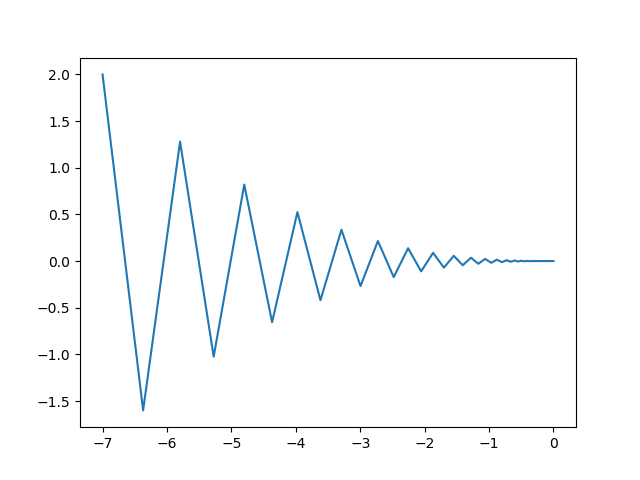
\includegraphics[scale = 0.5]{test1.png}
		\caption{SGDによる最適化}
		\label{test1}
	\end{center}
\end{figure}
図\ref{test1}は上の計算結果をプロットしたものである。確かに振動しつつ最小値に向かっており,非効率的な動きになっている。
\subsubsection{Momentum}
Momentumは次のような式で表すことができる:
\begin{eqnarray*}
\bm{v} &\leftarrow& \alpha \bm{v} - \eta \dfrac{\partial L}{\partial \bm{W}}\\
\bm{W} &\leftarrow& \bm{W}+\bm{v}
\end{eqnarray*}
SGDは$\alpha = 0.0$に対応する。$\alpha$はもとの速度を保とうとする効果(慣性)を与えている。また$\alpha < 1$ならばこの効果は指数的に減衰する。
\begin{lstlisting}
class Momentum:
	def __init__(self,lr = 0.01,momentum = 0.9):
		self.lr = lr
		self.momentum = momentum
		self.v = None
	
	def update_dict(self,params,grads):
		if self.v is None:
			self.v = {}
			for key,val in params.items():
				self.v[key] = np.zeros_like(val)
				
		
		for key in params.keys():
			self.v[key] = self.momentum*self.v[key]-self.lr*grads[key]
			params[key] += self.v[key]
	
	def update_array(self,params,grads):
		if self.v is None:
			self.v = np.zeros_like(params)
		for i in range(params.size):
			self.v[i] = self.momentum*self.v[i]-self.lr*grads[i]
			params[i] += self.v[i]
\end{lstlisting}
実装すると以上のようになる。{\texttt self.v}が初めに定義されていないことに注意。
\begin{figure}[htbp]
	\begin{center}
		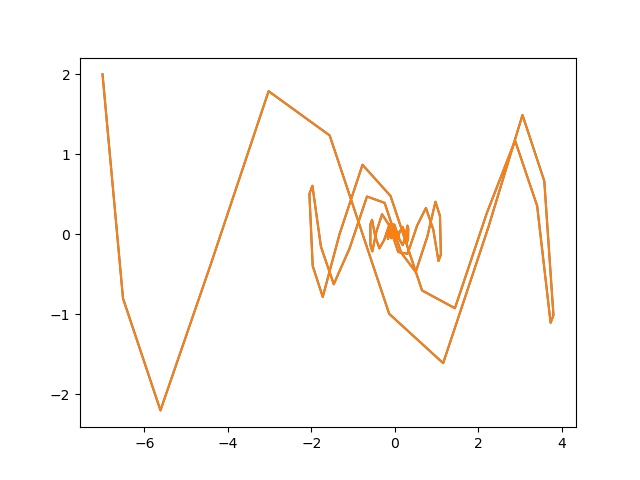
\includegraphics[scale = 0.5]{test2.png}
		\caption{Momentumによる最適化}
		\label{test2}
	\end{center}
\end{figure}
図\ref{test2}は上の計算結果をプロットしたものである。慣性を導入したことで滑らかに移動していることが確認できる。しかし今回は慣性が強いため最小値付近までたどり着いても収束するのに長い時間がかかっている。
\subsubsection{AdaGrad}
学習率$\eta$の大きさを適切に決めることが正しい学習には不可欠である。初めは大きくパラメータを動かし,次第にパラメータの動きを小さくさせるため,学習率を減衰させるという手法がよく用いられる。AdaGradは一つ一つのパラメータに対して個別に学習率を減衰させる。数式では以下のようになる:
\begin{eqnarray*}
\bm{h} &\leftarrow& \alpha \bm{h} + \eta \dfrac{\partial L}{\partial \bm{W}} \cdot \dfrac{\partial L}{\partial \bm{W}}\\
\bm{W} &\leftarrow& \bm{W}-\eta \dfrac{1}{\sqrt{\bm{h}}} \dfrac{\partial L}{\partial \bm{W}}
\end{eqnarray*}
まず$\cdot$は%これは後で変える
ベクトルを要素ごとに掛けてベクトルを生成する演算子である。よって$\bm{h}$はこれまでに経験した勾配の値をパラメータごとに二乗和として保存する。これによって,大きく更新されたパラメータの学習率は小さくなり,個別の学習率の減衰を実現することができる。\\
AdaGradを用いるとパラメータの更新量が$0$になってしまうことに注意。これを防ぐため,過去の勾配に指数的減衰を与えるRMSPropという手法がある。これを指数移動平均という。\\
AdaGradは以下のように実装することができる:
\begin{lstlisting}
class AdaGrad:
	def __init__(self,lr = 0.01):
		self.lr = lr
		self.h = None
		
	def update_dict(self,params,grads):
		if self.h is None:
			self.h = {}
			for key,val in params.items():
				self.h[key] = np.zeros_like(val)
				
		for key in params.keys():
			self.h[key] += grads[key]*grads[key]
			params[key] -= self.lr*grads[key]/(np.sqrt(self.h[key])+1e-7)
	
	def update_array(self,params,grads):
		if self.h is None:
			self.h = np.zeros_like(params)
		self.h += grads*grads
		params -= self.lr*grads/(np.sqrt(self.h)+1e-7)

\end{lstlisting}
これを用いて最適化した結果が図\ref{test3}である。
\begin{figure}[htbp]
	\begin{center}
		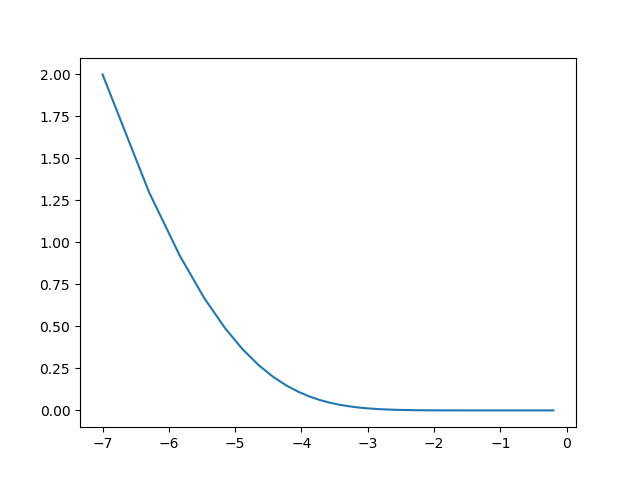
\includegraphics[scale = 0.5]{test3.png}
		\caption{Momentumによる最適化}
		\label{test3}
	\end{center}
\end{figure}
初めは$y$軸方向に大きな勾配を持っているが,それが抑制されて振動が軽減されている。
\subsubsection{Adam}
AdamはMomentumとAdaGradを融合させたような手法である。先ほどと同様に最適化を行うと,Momentumのように振動しつつ中心に向かうが,その振動はMomentumよりも軽減されている。これは学習率が適応的に更新されているためである。\\
なお,ハイパーパラメータのバイアス補正が行われているということもAdamの特徴である。
\subsubsection{どの更新手法を用いるか?}
$f(x,y) = \dfrac{1}{20} x^2 + y^2$を最小化するという目的に限ればAdaGradが最も効率的であるといえる。しかし考えたいタスクによって用いるべき最適化手法は当然異なり,それぞれの特徴を踏まえたうえで適切に選ぶ必要がある。
\subsubsection{MNISTデータセットによる更新手法の比較}
手書き数字認識を対象に,これまでの4つの手法を比較する。ネットワークの構成は$4$章と全く同じである。
\begin{figure}[htbp]
	\begin{center}
		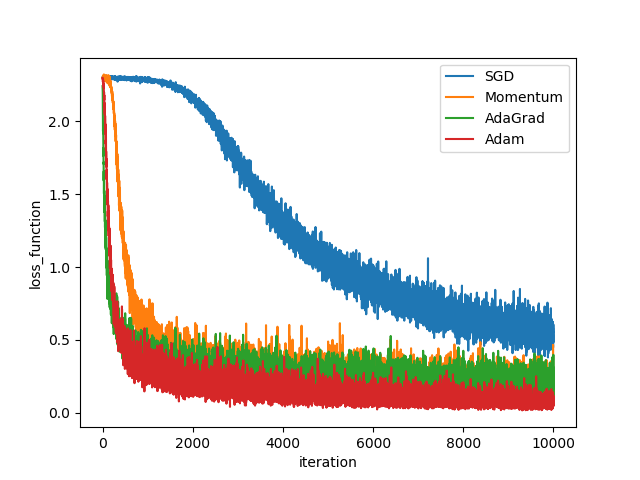
\includegraphics[scale = 0.5]{optimize_mnist.png}
		\caption{MNISTデータセットの学習の比較。}
		\label{optimize_mnist}
	\end{center}
\end{figure}
このタスクに関してはSGDよりも他の手法が早く学習できていることがわかる。SGDよりも他の手法の方が早く学習でき,時には最終的な認識性能も高くなるという傾向がある。AdaGradが最も効率的に学習しているようだが,ハイパーパラメータやニューラルネットワークの構造によって結果は変化するということに注意。

\subsection{重みの初期値}
重みの初期値がニューラルネットワークの学習の成否を分けることが実際によくある。またニューラルネットワークの学習を速やかに進めるためにも初期値の設定は重要である。
\subsubsection{重みの初期値を$0$にすることの問題点}
過学習が生じているときには重みの値が大きくなっていることが多い。よって重みパラメータの値が小さくなるように学習を行えば過学習を防ぐことができると期待できる。この手法をWeight decayという。\\
重みの値が小さくなるように,初期値をすべて$0$にすることも考えられるが,これでは重みの更新が生じず,したがって学習が進まなくなってしまう。学習を行う上では,重みの対称的な構造を崩すことが重要になる。
\subsubsection{隠れ層のアクティベーション分布}
活性化関数の出力の分布をアクティベーション分布という。以下のヒストグラムは,$5$つの隠れ層を持つニューラルネットワークに対してランダムに生成した入力データを流し込んだ時のアクティベーション分布を表したものである。それぞれ重みパラメータを標準偏差$0.01$から$1.0$としたときのアクティベーション分布を示している。
\begin{figure}[htbp]
	\begin{center}
		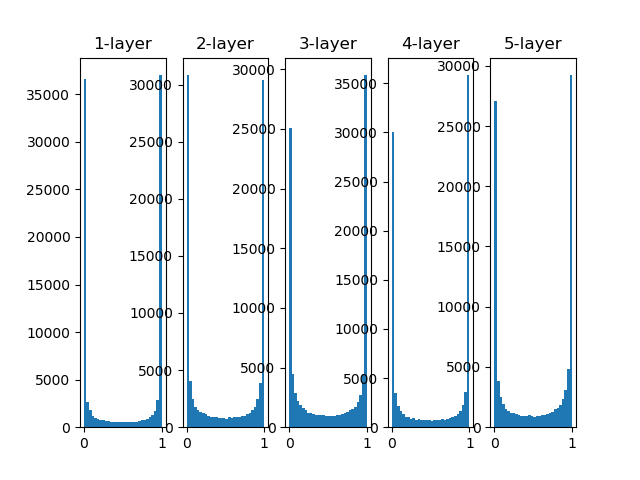
\includegraphics[scale = 0.5]{histogram1.png}
		\caption{標準偏差$1.0$のガウス分布を用いたときのアクティベーション分布}
		\label{histogram1}
	\end{center}
\end{figure}
\begin{figure}[htbp]
	\begin{center}
		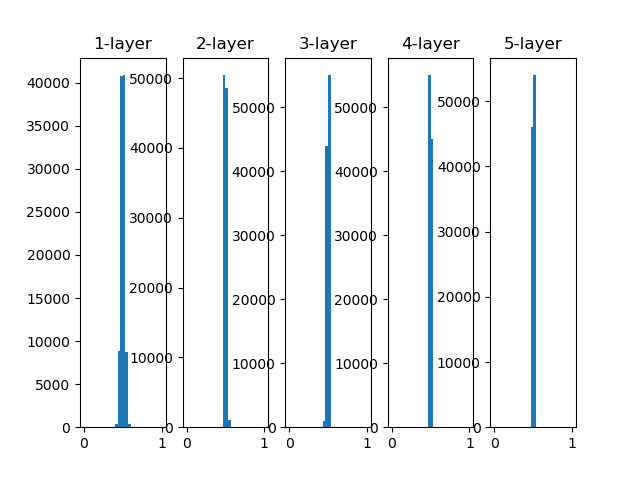
\includegraphics[scale = 0.5]{histogram2.png}
		\caption{標準偏差$0.01$のガウス分布を用いたときのアクティベーション分布}
		\label{histogram2}
	\end{center}
\end{figure}
\begin{figure}[htbp]
	\begin{center}
		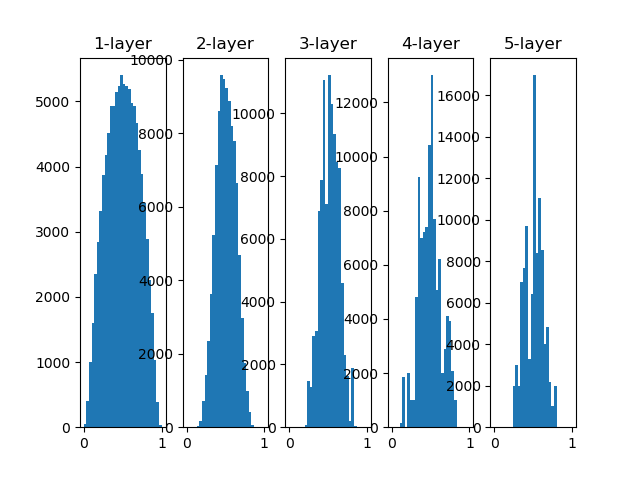
\includegraphics[scale = 0.5]{histogram3.png}
		\caption{標準偏差$0.1$のガウス分布を用いたときのアクティベーション分布}
		\label{histogram3}
	\end{center}
\end{figure}
標準偏差$1.0$のときのアクティベーション分布を見ると,多くが$0$と$1$に偏っている。このとき損失関数の勾配はシグモイド関数の振る舞いから考えて小さくなると考えることができる(勾配消失)。\\
標準偏差$0.01$のときのアクティベーション分布はほとんどが$0.5$に近い値をとっている。これは勾配消失の問題は生じないが,ほとんどのニューロンが同じ値を示すのならばそれらは1つのニューロンで表すことができる。つまり表現力の問題が生じる。\\
標準偏差$0.1$のときのアクティベーション分布は適度な広がりを保っている。これによりシグモイド関数の表現力が妨げられることもなく,うまく学習が進む。これは前層のニューロン数を$n$としたとき,初期値の分散を$1/\sqrt n$程度にとるXavierの初期値を用いている。\\
なお,上位層の分布の形状がいびつになったのは{\texttt tanh}関数ではなく{\texttt sigmoid}関数を用いたためである。活性化関数としては原点対象であることが望ましいとされている。

\subsubsection{ReLUの場合の重み初期値}
Xavierの初期値は活性化関数が線形であることを前提に導かれている。{\texttt sigmoid}関数や{\texttt tanh}関数は左右対称で中央付近が線形関数とみなせるためXavierの初期値が適している。\\
一方ReLUを用いるときにはReLUに特化したHeの初期値を用いることが推奨されている。これは前層のノード数が$n$個であるとき,$\sqrt{\dfrac{2}{n}}$を標準偏差とするガウス分布を用いる初期値である。
\subsubsection{MNISTデータセットによる重み初期値の比較}
MNISTデータセットに対し重みの初期値の与え方を変えたときに,学習の進み方がどのように変わるかを調べたところ,ReLUを用いたときにはHeの初期値が最も効率的に学習が進む。

\subsection{Batch Normalization}
各層で適度な広がりを持つように強制的にアクティベーション分布を調整する手法がBatch Normalizationである。
\subsubsection{Batch Normalizationのアルゴリズム}
Batch Normには次の利点がある:
\begin{enumerate}
\item 学習を早く進行させることができる
\item 初期値にそれほど依存しない
\item 過学習を抑制する
\end{enumerate}
これは各層においてBatch Normレイヤを挿入することで,データ分布の正規化を行う。具体的な計算は以下のようになる:
\begin{eqnarray*}
\mu_{\rm B} &\leftarrow& \dfrac{1}{m} \sum_{i = 1}^{m} x_i\\
\sigma_{\rm B}^2 &\leftarrow& \dfrac{1}{m} \sum_{i=1}^{m} (x_i - \mu_{\rm B})^2\\
\hat{x}_i &\leftarrow& \dfrac{x_i - \mu_{\rm B}}{\sqrt{\sigma_{\rm B}^2+\epsilon}}\\
y_i &\leftarrow& \gamma \hat{x}_i + \beta
\end{eqnarray*}
ここで$\epsilon$は発散を防ぐための小さなパラメータであり,また$\gamma$と$\beta$は学習によって適した値に調整されるパラメータである。

\subsubsection{Batch Normalizationの逆伝播の導出}
https://kratzert.github.io/2016/02/12/understanding-the-gradient-flow-through-the-batch-normalization-layer.htmlに基づいてBatch Normの逆伝播を導出する。

\subsubsection{Batch Normalizationの評価}
Batch Normを利用した方が学習の進みが早くなる。また重みの初期値を適当に設定してもうまく学習が進むことが多い。

\subsection{正則化}
過学習を抑制するための手段として正則化というものがある。
\subsubsection{過学習}
過学習が生じる原因として,主に次の2つを上げることができる:
\begin{enumerate}
\item パラメータを大量に持ち,表現力が高いモデルであること
\item 訓練データが少ないこと
\end{enumerate}
がある。実際にMNISTのデータに対して訓練データを$300$個にし,$7$層のニューラルネットワークを用いたところ,訓練データに対する認識制度は$100\%$であったが,テストデータに対しては$100\%$からは大きな隔たりがある。
\subsubsection{Weight decay}
Weight decayは大きな重みパラメータを持つことにペナルティーを科すことで過学習を抑制するという手法である。つまり損失関数に対し,L2ノルムに比例する$\dfrac{1}{2} \lambda \bm{W}^2$という項を加えることでこれを実現できる。よって重みの勾配を計算するときには誤差逆伝播法による結果に加えて$\lambda \bm{W}$を考慮する必要がある。
ここでL1ノルム,L2ノルム,L$\infty$ノルムのいずれを用いてもよいことに注意。それぞれの定義は以下のようになる:
\begin{eqnarray*}
|\bm{W}|_1 &=& |w_1|+|w_2|+\cdots+|w_n|\\
|\bm{W}|_2 &=& \sqrt{w_1^2+w_2^2+\cdots+w_n^2}\\
|\bm{W}|_{\infty} &=& \max(w_1,w_2,\cdots,w_n)
\end{eqnarray*}
これを利用して先ほどと同様の学習を行うと,テストデータに対する認識制度が向上する。また訓練データに対する認識制度が$100\%$に達しないということにも注意。
\subsubsection{Dropout}
Weight decayは単純な方法で,ある程度過学習を抑制することができる。しかしニューラルネットワークのモデルが複雑になるとDropoutという手法が良く用いられるようになる。\\
Dropoutはニューロンをランダムに消去しながら学習するという手法である。
実際にこれを適用して学習をすることで,過学習が抑制される。
\subsection{ハイパーパラメータの検証}
各層のニューロン数やバッチサイズ,学習率やWeight decai(の$\lambda$)などがハイパーパラメータと呼ばれる。これは学習によって変化することのない値であり,うまく決定する必要がある。ここでは効率的にハイパーパラメータの値を探索する方法について説明する。
\subsubsection{検証データ}
ハイパーパラメータの性能を評価するときにはテストデータを利用してはならない。なぜならばハイパーパラメータの値がテストデータに対して過学習を起こすことになるためである。よってハイパーパラメータ専用の確認データ(検証データ)が必要になる。訓練データとテストデータしかない場合は,訓練データの中から$20\%$程度を先に分離して検証データとすればよい。
\begin{lstlisting}
>>> (x_train,t_train),(x_test,t_test) = load_mnist()
>>> x_train,t_train = shuffle_dataset(x_train,t_train)

>>> validation_rate = 0.20
>>> calidation_num = int(x_train.shape[0]*validation_rate)
>>> validation_num = int(x_train.shape[0]*validation_rate)

>>> x_val = x_train[:validation_num]
>>> t_val = t_train[:validation_num]
>>> x_train = x_train[validation_num:]
>>> t_train = t_train[validation_num:]
\end{lstlisting}
ここで{\texttt shuffle\_dataset()}という関数を利用している。この定義は以下のようになっている:
\begin{lstlisting}
def shuffle_dataset(x, t):
    permutation = np.random.permutation(x.shape[0])
    x = x[permutation,:] if x.ndim == 2 
    	else x[permutation,:,:,:]
    t = t[permutation]

    return x, t
\end{lstlisting}
{\texttt x}の次元数によって場合分けをしていること,スライシングの表記がいまいちよくわかっていない。
\subsubsection{ハイパーパラメータの最適化}
ハイパーパラメータの最適化を行う上で重要なポイントは,ハイパーパラメータの最適値が存在する範囲を徐々に絞り込んでいくということにある。そのときにはグッリドサーチなどの規則的な探索よりも,ランダムに(対数スケールで)サンプリングして得られた認識精度を観察して最適値を絞り込むほうが効率が良い。これは複数あるハイパーパラメータのうち,最終的な認識精度に与える影響度合いがハイパーパラメータごとに異なるためである。\\
以上の手順をまとめると以下のようになる:
\begin{enumerate}
\item ハイパーパラメータの範囲を設定する
\item 設定されたハイパーパラメータの範囲から,ランダムにサンプリングする
\item 1.でサンプリングされたハイパーパラメータの値を使用して学習を行い,検証データで認識精度を評価(ただしエポックは小さく設定)
\item 1.と2.をある回数($100$回など)繰り返し,それらの認識精度の結果から,ハイパーパラメータの範囲を狭める
\end{enumerate}
より洗練された手法としてはベイズ最適化がある。これを用いるとより厳密に効率よく最適化を行うことができる。

\subsubsection{ハイパーパラメータ最適化の実装}
{\texttt weight\_decay = 10**np.random.uniform(-8,-4)}のような表記を用いると,対数スケールでランダムにサンプリングをすることができる。このように得られた$20$程度のサンプルのうち,認識精度の高いものについてハイパーパラメータの範囲を調べる。ここからより範囲を狭めることができる。
\subsection{まとめ}
パラメータの更新方法や,重みの初期値の与え方,Batch NormalizationやDropoutなど,現代のニューラルネットにとっては書くことのできない技術になっている。またこれらは最先端のDLにおいても頻繁に利用されている。

%%%%%%%%%%%%%%%%%%%%%%%%%%%%%%%%%%%%%%
%%%%%%%%%%%%%%%%%%%%%%%%%%%%%%%%%%%%%%%
%%%%%%%%%%%%%%%%%%%%%%%%%%%%%%%%%%%%%%%
\end{document}
